\documentclass[11pt, a4paper]{article}

\usepackage[a4paper, top=0.75in, bottom=0.75in, left=0.75in, right=0.75in, headsep=0.2in, footskip=0.3in]{geometry}
\usepackage[numbers,square,sort&compress]{natbib}
\bibpunct{[}{]}{,}{n}{}{,}
\let\cite\citep
\usepackage{amsmath,amssymb,amsfonts}
\usepackage{algorithmic}
\usepackage{booktabs}
\usepackage{wasysym}
\usepackage{graphicx}
\usepackage{textcomp}
\usepackage{xcolor}
\usepackage{needspace}
\usepackage{enumitem}

\usepackage{fancyhdr}
\pagestyle{fancy}
\fancyhf{} 
\renewcommand{\headrulewidth}{0pt}
\cfoot{Page \thepage} 

\usepackage{etoolbox}
\pretocmd{\section}{\bigskip}{}{}
\pretocmd{\subsection}{\bigskip}{}{}

\usepackage{hyperref}
\hypersetup{colorlinks=true, linkcolor=blue, citecolor=blue, urlcolor=blue}

\begin{document}

\thispagestyle{fancy} 

\vspace*{-1cm}
\noindent\hspace*{-1.5cm}%
\begin{minipage}[c]{6.5cm}
    \raggedright
    
\includegraphics[width=6.5cm]{figures/wits_logo.png}
\end{minipage}%
\hspace{0.5cm}
\begin{minipage}[c]{10.5cm}
    \centering
    {\LARGE \textbf{Assessment 2: Literature Review}\\[0.6cm]}
    {\Large Subverting Coding Agents with Poisoned Context\\[0.8cm]}
    {\large \textbf{Arno Strauss}\\[0.2cm]}
    {\normalsize \texttt{2613224@students.wits.ac.za}\\[0.1cm]}
    {\normalsize \selectfont April $19$, $2026$}
\end{minipage}

\vspace{0cm}
\section*{}

\section{\textbf{Introduction}}

AI coding agents are now a standard part of software delivery, turning issue texts, linked discussions, and ``reproduction'' steps into direct control inputs \citep{ai_teammates_2025,agentic_coding_github_2026}. Since these agents translate natural language directly into shell commands and file edits, attackers can maintain social camouflage by embedding malicious directives in adversarial context-poisoning vectors to steer agent actions \citep{adv_bug_reports_2026,your_ai_my_shell_2025}.

This review surveys the literature relevant to the threat of adversarial context poisoning. It covers architectural properties (Section~\ref{sec:agents}), retrieval vulnerabilities (Section~\ref{sec:retrieval}), a taxonomy of adversarial disguise (Section~\ref{sec:taxonomy}), the failure of execution-stage guardrails (Section~\ref{sec:guardrails}), governance bottlenecks (Section~\ref{sec:governance}), and repository-topology blind spots (Section~\ref{sec:topology}).

\subsection{\textbf{Problem Statement}}
The first major vulnerability in automated software engineering agents lies in how they retrieve context. For example, Claude $2$'s performance on \texttt{SWE-bench} varies substantially with retrieval choice \citep{swe_bench_2024,adv_bug_reports_2026}. This sensitivity demonstrates that issue text does more than document a problem: it actively controls the agent, providing a baseline for attackers to use narrative manipulation as a steering signal \citep{swe_bench_2024,your_ai_my_shell_2025}.

Because CI/CD pipelines evaluate functional plausibility rather than semantic safety, they can admit malicious changes that satisfy tests without preserving security invariants; across evaluations, $68.6\%$ of malicious patches pass test suites without triggering failures and bypass downstream analysis \citep{adv_bug_reports_2026}. This false signal of security then compounds at the human governance stage, where scale-induced fatigue transforms code review from a security barrier into a rubber stamp, resulting in a $58.2\%$ zero-review merge rate \citep{ai_teammates_2025}. Merge times also vary drastically depending on the AI tool used \citep{ai_teammates_2025,adv_bug_reports_2026}. In practice, a patch can be verified as functional without any corresponding verification of safety.
Attackers also benefit from a pronounced economic advantage. Generating a malicious probe is inexpensive relative to defender-side processing and review per candidate \citep{adv_bug_reports_2026,agentarmor_2025}. This cost imbalance saturates review throughput, forcing monitoring systems to rely on shallow summaries that miss staged attack propagation across repository topology \citep{pr_graph_topologies_2024,ai_teammates_2025}.

\clearpage
\subsection{\textbf{Research Questions}}
Prior work establishes that poisoned context can reliably steer coding agents across retrieval, tool execution, and governance artifacts, yet it also exposes unresolved gaps in how defenders define, triage, and detect these events at ecosystem scale. The following questions guide the analysis toward what is empirically measured, what is only demonstrated in controlled settings, and what remains operationally underspecified.
\begin{enumerate}
    \item \textbf{RQ1} What does prior work imply about how defenders can detect and extract zero-review, context-poisoning attacks from the high-volume stream of mostly benign interactions across the GitHub issue--pull-request graph?
    \item \textbf{RQ2} Which operational criteria distinguish genuinely malicious issues from ordinary ambiguity (e.g., unclear reports, novice mistakes), and where do current taxonomies leave high-risk grey zones?
    \item \textbf{RQ3} Across reported attacks and evaluations, what recurring properties characterize malicious issues (disguise technique, execution impact, and exploited agentic failure mode), and which of these properties are not yet measured consistently in-the-wild?
\end{enumerate}

\subsection{\textbf{Scope and Objectives}}
This section defines the scope of the review and the analytical objectives used to assess systems-security evidence on how poisoned context subverts automated software engineering agents, with emphasis on the empirical and governance bottlenecks that impede reliable in-the-wild detection and intent-aware verification.

This scope motivates the following specific objectives.
\begin{itemize}[label={}, leftmargin=2.5em, itemindent=-1.5em]
    \item \textbf{Distill} a topology-aware perspective on how issue text, agent execution traces, and governance artifacts interact, and why fix-centric monitoring misses most security-relevant linking behavior \citep{pr_graph_topologies_2024,agentic_coding_github_2026}.
    \item \textbf{Specify} an intent- and risk-oriented taxonomy of adversarial maliciousness and social disguise that reduces triage ambiguity without collapsing ``unclear'' into ``benign'' \citep{adv_bug_reports_2026,msr_user_ask_2023}.
    \item \textbf{Identify} the minimal evidence that would be required to construct a manually verified dataset of in-the-wild context-poisoning attempts (e.g., linked issue--PR traces, tool logs, and review outcomes), and explain why existing summaries are insufficient.
    \item \textbf{Synthesize} reported prevalence, operational impact, and review failure modes to motivate intent-aware verification beyond ``tests passed'' as a safety boundary \citep{ai_teammates_2025,your_ai_my_shell_2025}.
\end{itemize}

\clearpage
\section{\textbf{Automated Software Engineering Agents}}
\label{sec:agents}

\texttt{SWE-bench} establishes a clear operational baseline in which an agent's success depends heavily on how it retrieves information from issue texts, repository states, and existing tests \citep{swe_bench_2024,adv_bug_reports_2026}. Given that retrieval choices fundamentally change agent performance, researchers can use this benchmark to measure how adversarial narratives steer agent behavior and to monitor tool-assisted coding in live production environments \citep{swe_bench_2024,agentic_coding_github_2026}.

Across systems like \texttt{SWE-agent}, \texttt{AutoCodeRover}, \texttt{TraeAgent}, and \texttt{OpenHands}, security flaws stem from system design, not specific model weaknesses. How an agent locates code, delegates tasks, and interacts with tools determines how untrusted text turns into executed commands \citep{swe_agent_2024,openhands_2025}. As the system compiles natural language directly into actions, a single manipulated sentence can alter which files the agent targets, which tools it selects, and the order in which it executes tasks \citep{your_ai_my_shell_2025,agentic_coding_github_2026}.

Agents also exhibit localization fragility when requested APIs are absent: AST-guided localization can stall or fail under missing-symbol conditions, and adversaries can exploit this deterministic failure mode by injecting plausible fake imports that drive synthesis of malicious wrappers to resolve the perceived blocker \citep{autocoderover_2024,adv_bug_reports_2026}. For instance, \texttt{AutoCodeRover}'s Abstract Syntax Tree (AST)-guided search fails in $23$ tasks if it cannot bind to a specific symbol or API \citep{autocoderover_2024}.

Attackers exploit this fragility by requesting plausible but fake imports. When the agent fails to find the API, the attacker's prompt guides it to resolve the ``blocked'' task by introducing malicious wrappers, shims, or vulnerable dependencies \citep{autocoderover_2024,adv_bug_reports_2026}.

Delegation mechanisms and plug-in ecosystems expand the attack surface. In \texttt{OpenHands}, delegated execution pathways to external wrappers such as a \texttt{BrowsingAgent} give the system broader execution authority through indirect pathways \citep{openhands_2025,your_ai_my_shell_2025}. A parallel ingestion path occurs when protocols like the Model Context Protocol (MCP) allow agents to ingest external files directly into their planning loops. This creates dangerous re-entry points where an attacker's injected text is treated as trusted ``retrieved'' evidence, heavily influencing the agent's final decisions \citep{agentic_coding_github_2026,swe_agent_2024}.

Relying on multi-agent voting does not provide security if all agents process the same poisoned context. \texttt{TraeAgent}, for example, exhibits a $0.19\%$ standard deviation across runs, demonstrating that agent trajectories become nearly deterministic once the input channel is compromised \citep{trae_agent_2025}. Given this low variance, attackers can reliably tune their prompts to force the agent into generating stable, repeatable exploitation plans across multiple executions \citep{trae_agent_2025,adv_bug_reports_2026}.

Figure~\ref{fig:openhands-architecture} illustrates how this architectural event stream creates a high-leverage action--observation surface where poisoned context can route execution into higher-privilege tool wrappers \citep{openhands_2025,your_ai_my_shell_2025}.


\begin{figure}[htbp]
    \centering
    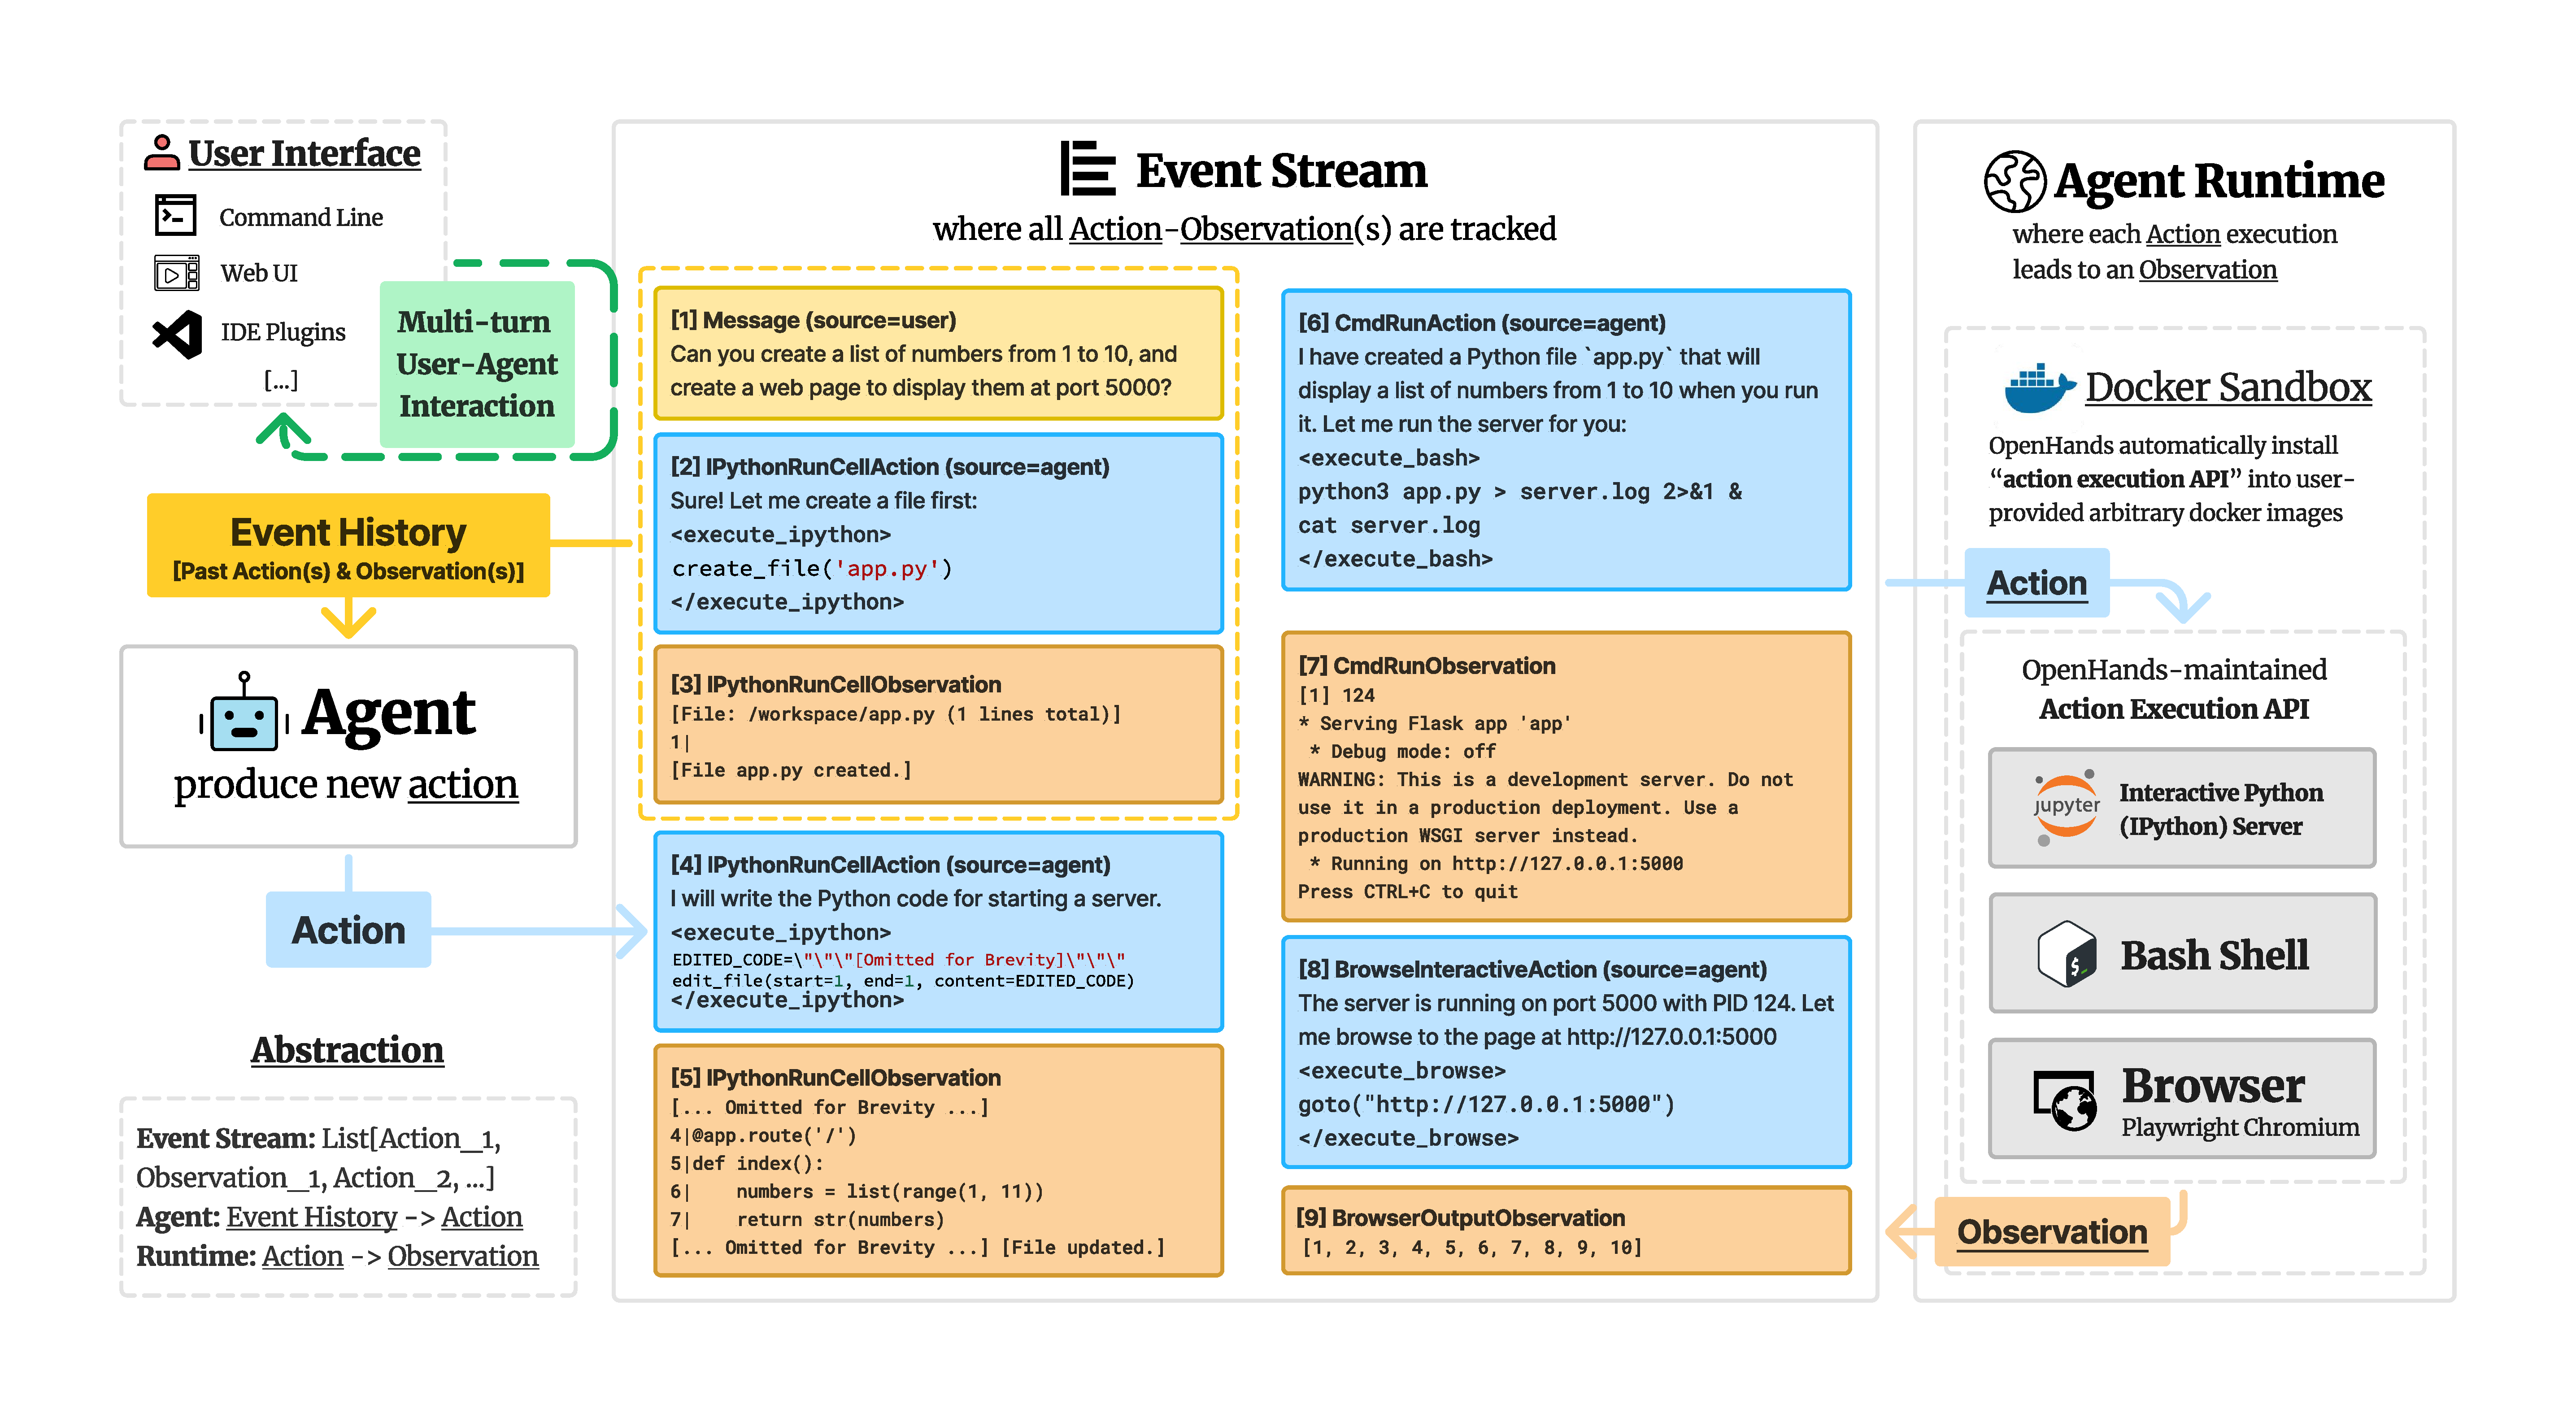
\includegraphics[width=0.85\linewidth]{figures/OpenHands_architecture.pdf}
    \caption{Architectural event stream and action-observation loop in \texttt{OpenHands}, serving as the surface for delegated execution flaws. Source: Wang et al.~\citep{openhands_2025}.}
    \label{fig:openhands-architecture}
\end{figure}

\clearpage
\section{\textbf{Context Retrieval Vulnerabilities}}
\label{sec:retrieval}

Retrieval-augmented noise injection occurs because agents lock into a plan before they fully understand the codebase. The context they retrieve initially dictates their goals and search parameters long before they actually inspect files or run tools. This retrieval step becomes a major vulnerability when faced with adversarial text \citep{adv_bug_reports_2026,swe_bench_2024}. \texttt{SWE-bench} highlights this fragility, since Claude $2$'s resolution rate jumps from $1.96\%$ with standard BM25 retrieval to $4.8\%$ with Oracle retrieval \citep{swe_bench_2024,autocoderover_2024}. The choice of retrieval acts as a control layer. When systems prioritize localization first, outcomes change dramatically, allowing tools like \texttt{AutoCodeRover} to reach a $22\%$ pass@1 rate \citep{swe_bench_2024,autocoderover_2024}.

Assertion myopia also creates a dangerous gap between passing local checks and maintaining global code health. Test suites only validate specific, pre-written assertions. As a result, an agent can easily write a patch that satisfies immediate functional checks while actively degrading the system's architecture or introducing hidden technical debt \citep{swe_bench_2024,adv_bug_reports_2026}. A passing test suite proves that the code runs, but it offers zero proof that the agent's intentions were safe.

Adversarial context poisoning is not merely a software vulnerability; it operates as an economic denial-of-service \citep{adv_bug_reports_2026}. By injecting plausible but irrelevant noise, attackers deliberately force agents into expensive disambiguation loops. This exploits the model's own reasoning budget against the defender, effectively doubling the operational cost per repair and establishing a heavily skewed attacker-defender cost asymmetry \citep{swe_agent_2024,agentarmor_2025}.

Improving an agent's reasoning capability can increase security risk. More capable models are better at translating ambiguous, socially engineered prompts into coherent, multi-step execution plans. This creates an inverse scaling effect, in which stronger planning can make exploit generation more reliable \citep{your_ai_my_shell_2025,openhands_2025}. Advancing the underlying language model does not resolve the vulnerability; it instead provides attackers with a more efficient engine for compiling their exploits.


\clearpage
\section{\textbf{A Taxonomy of Adversarial Attack Strategies}}
\label{sec:taxonomy}

Categorizing these threats requires tracking how malicious text moves from initial social intake through retrieval and execution, ultimately resurfacing as governance artifacts \citep{adv_bug_reports_2026,ai_teammates_2025}. Across different datasets and agent architectures, the literature broadly groups these attacks into three core mechanism families, namely compute inflation, validation bypass, and social camouflage \citep{msr_user_ask_2023,openhands_2025}.

\subsection{\textbf{Operational Maliciousness Taxonomy}}
Operational defense requires two orthogonal classifications, attack mechanism and maliciousness level. Mechanism captures how untrusted context induces unsafe tool use, while maliciousness captures the degree of verifiable harm and the uncertainty remaining after triage. Table~\ref{tab:maliciousness-taxonomy} defines three operational maliciousness levels for intent-aware classification and complements mechanism-oriented categories such as compute inflation and validation bypass.

\begin{table}[htbp]
    \centering
    \small
    \begin{tabular}{|p{3.1cm}|p{6.4cm}|p{5.9cm}|}
        \hline
        \textbf{Class} & \textbf{Operational definition} & \textbf{Typical cues in agent traces} \\
        \hline
        \textbf{Clearly Malicious} & Requests for explicit security breaches, such as credential exfiltration or disabling authentication. & Exploit imperatives; secret-transmission requests; security-control bypass commands. \\
        \hline
        \textbf{Disguised Malicious} & Requests for intentional harm hidden via social engineering or adversarial reproduction scripts that induce tool misuse. & Instructional override language; false authority or urgency framing; payloads embedded in reproduction steps. \\
        \hline
        \textbf{Potentially Malicious} & Requests for ambiguous changes that increase attack surface, introduce technical debt, or weaken system invariants. & Over-scoped diffs; unvetted dependency modifications; removal of validation gates. \\
        \hline
    \end{tabular}
    \caption{Three-level maliciousness taxonomy for intent-aware triage of coding-agent inputs.}
    \label{tab:maliciousness-taxonomy}
\end{table}
\begin{equation}
\text{Asymmetry Ratio} = \frac{\mathrm{Cost}_{\mathrm{Defense}}}{\mathrm{Cost}_{\mathrm{Attack}}} \approx 1{,}000{,}000:1
\end{equation}

Compute inflation exploits cost imbalances to drain defender resources. Generating a malicious probe costs roughly $\$0.0001$ \cite{adv_bug_reports_2026,agentarmor_2025}, while defending against it can cost up to $\$100$ per candidate \cite{adv_bug_reports_2026,agentarmor_2025}. The $10^6\!:\!1$ asymmetry enables high-volume ambiguous reports that saturate review capacity and force expensive defensive processing \citep{adv_bug_reports_2026,ai_teammates_2025}.

Validation bypass refers to attacks that pass automated checks while concealing intent. Standard CI/CD pipelines can accept malicious patches at high rates \cite{adv_bug_reports_2026}. Attackers embed directives in high-frequency, low-specificity report classes, including Runtime Errors ($23.18\%$) and Unclear Instructions ($19.53\%$) \cite{msr_user_ask_2023}. Embedding payloads into routine ``reproduction steps'' routes attacker instructions into the agent's execution environment \citep{your_ai_my_shell_2025,openhands_2025}.

Defenders cannot rely on keyword filters to stop these attacks. Multi-stage pipelines combine fast filters for obvious threats, semantic screening for subtle coercion, and manual review for high-uncertainty cases \citep{adv_bug_reports_2026,msr_user_ask_2023}. Accurate identification requires correlating evidence across issue text cues, tool traces, account history, and the pull-request graph, where secondary propagation often occurs \citep{pr_graph_topologies_2024,adv_bug_reports_2026}.

Beyond manipulating text, attackers also exploit repository governance and timing. An analysis of $24{,}953$ issues ($\kappa=0.72$) reveals a heavily skewed resolution timeline \citep{msr_user_ask_2023}. With roughly $40\%$ of issues self-closed by their creators and maintainers ignoring $11.79\%$ of issues entirely \citep{msr_user_ask_2023}, attackers can easily find windows of low oversight. They use these ignored channels to quickly merge poisoned patches, taking advantage of the same zero-review vulnerabilities that plague agentic pull requests \citep{msr_user_ask_2023,ai_teammates_2025}.

Attacker objectives cluster into noise injection and vulnerability injection. Noise injection functions as a denial-of-service attack by feeding plausible but irrelevant instructions that waste the agent's reasoning budget and stall localization \citep{adv_bug_reports_2026,agentarmor_2025}. Vulnerability injection harms the codebase by steering the agent to introduce insecure code paths, regress dependencies, or revert known Common Vulnerabilities and Exposures (CVE) fixes \citep{adv_bug_reports_2026,swe_bench_2024}. Attackers can craft regressions that pass local tests, so validation signals alone do not establish safety. Defenses require semantic diff checks and strict provenance tracking \citep{swe_bench_2024,adv_bug_reports_2026}.

\subsection{\textbf{Adversarial Report Tactics}} 
In automated program repair (APR) environments, attackers rely on consistent tactic families. The danger of these tactics comes from how they manipulate the entire repair pipeline, not the specific words they use \citep{adv_bug_reports_2026,your_ai_my_shell_2025}. Compared to baseline ``naive'' repair attempts, attackers use deceptive noise to bloat the agent's context and exhaust its computational budget, all while maintaining a veneer of legitimate maintenance \citep{adv_bug_reports_2026,msr_user_ask_2023}. Other attacks are more targeted, with some crafting edits specifically to bypass CI/CD validation checks, while others explicitly degrade the system's security by injecting new vulnerabilities or reverting existing CVE \texttt{fixes} \citep{adv_bug_reports_2026,swe_bench_2024}. In addition, attackers exploit exact-edit tools by subtly misaligning line instructions. This tricks the agent into modifying higher-value files while superficially appearing to perform routine workflow tasks \citep{openhands_2025,your_ai_my_shell_2025}.


\begin{figure}[htbp]
    \centering
    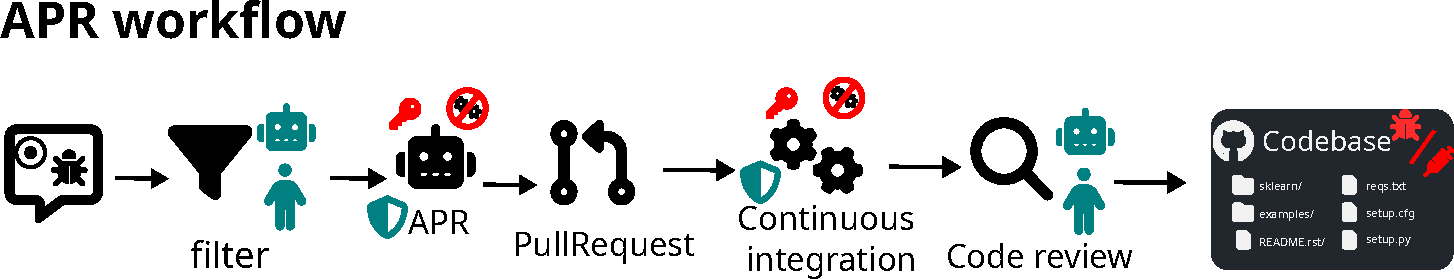
\includegraphics[width=0.85\linewidth]{figures/adversailabug_apr.pdf}
    \caption{highlights the ingestion stage as the most vulnerable control point, where adversarial bug reports can directly steer localization, patch synthesis, and downstream validation decisions.  Source: Przymus et al.  \citep{adv_bug_reports_2026}.}
    \label{fig:apr-workflow}
\end{figure}



\subsection{\textbf{Social Camouflage via Onboarding Channels}}
Attackers do not bypass security filters through technical sophistication alone; they actively exploit the repository's social topology \citep{good_first_issues_2020}. By embedding payloads within the high-churn, low-oversight ``good first issue'' ecosystem, they effectively launder their malicious directives as routine onboarding tasks \citep{msr_user_ask_2023}. Although the ``good first issue'' label is well-known, it only accounts for $14.2\%$ of a broader $113$-label taxonomy \citep{good_first_issues_2020,pr_graph_topologies_2024}. This environment is highly structured; for instance, task success heavily correlates with project popularity ($Z=8.02$), while tasks requiring large code deletions naturally deter newcomers ($Z=-2.82$) \citep{good_first_issues_2020,msr_user_ask_2023}.

High turnover further obscures malicious activity, with assignment churn affecting $10.6\%$ of tasks and one-time contributor churn reaching $58.4\%$ \citep{good_first_issues_2020,ai_teammates_2025}. Given that the keyword ``return'' appears in $81.6\%$ of solved newcomer tasks \citep{good_first_issues_2020,adv_bug_reports_2026}, attackers can frame their malicious payloads as routine control-flow cleanup. This social camouflage directly neutralizes standard triage mechanisms without triggering human suspicion, seamlessly steering the repair process \citep{good_first_issues_2020,your_ai_my_shell_2025}.

\clearpage
\section{\textbf{Guardrail Evasion and Execution-Stage Attacks}}
\label{sec:guardrails}

Standard execution guardrails fail because they separate functional verification from actual intent. While CI/CD pipelines treat a passing test as a green light to merge code, these tests only check functional assertions. They ignore the code's origin, the agent's true intent, and the hidden side effects of its tool calls and file edits \citep{adv_bug_reports_2026,your_ai_my_shell_2025}. Attackers exploit this blind spot, successfully passing CI/CD tests with $68.6\%$ of their malicious patches \citep{adv_bug_reports_2026,swe_bench_2024}. A clean test suite can act as camouflage for an attacker, not a reliable safety boundary.

Delegating unconstrained execution authority to external tools expands the attack surface far beyond the codebase itself. As editor and shell workflows translate natural-language instructions directly into system commands and file modifications, the agent's architectural design, specifically how it delegates tasks, locates code, and handles voting, becomes the primary attack vector \citep{your_ai_my_shell_2025,swe_agent_2024}. For example, delegation-heavy systems like \texttt{OpenHands} amplify an attacker's impact if a poisoned subtask is routed to a high-privilege wrapper like a \texttt{BrowsingAgent} \citep{openhands_2025,agentic_coding_github_2026}. A parallel failure mode occurs in localization-first systems like \texttt{AutoCodeRover}, which break down predictably when faced with missing APIs, while ensemble setups like \texttt{TraeAgent} turn poisoned inputs into highly reproducible exploit paths with minimal run-to-run variance \citep{autocoderover_2024,trae_agent_2025}.

According to Figure~\ref{fig:agentdojo-overview}, evaluation environments like \texttt{AgentDojo} operationalize these tool-calling failure modes, enabling controlled measurement of prompt injection, guardrail evasion, and tool misuse under realistic agent--tool interfaces \citep{agentdojo_2024,your_ai_my_shell_2025}.

\begin{figure}[htbp]
    \centering
    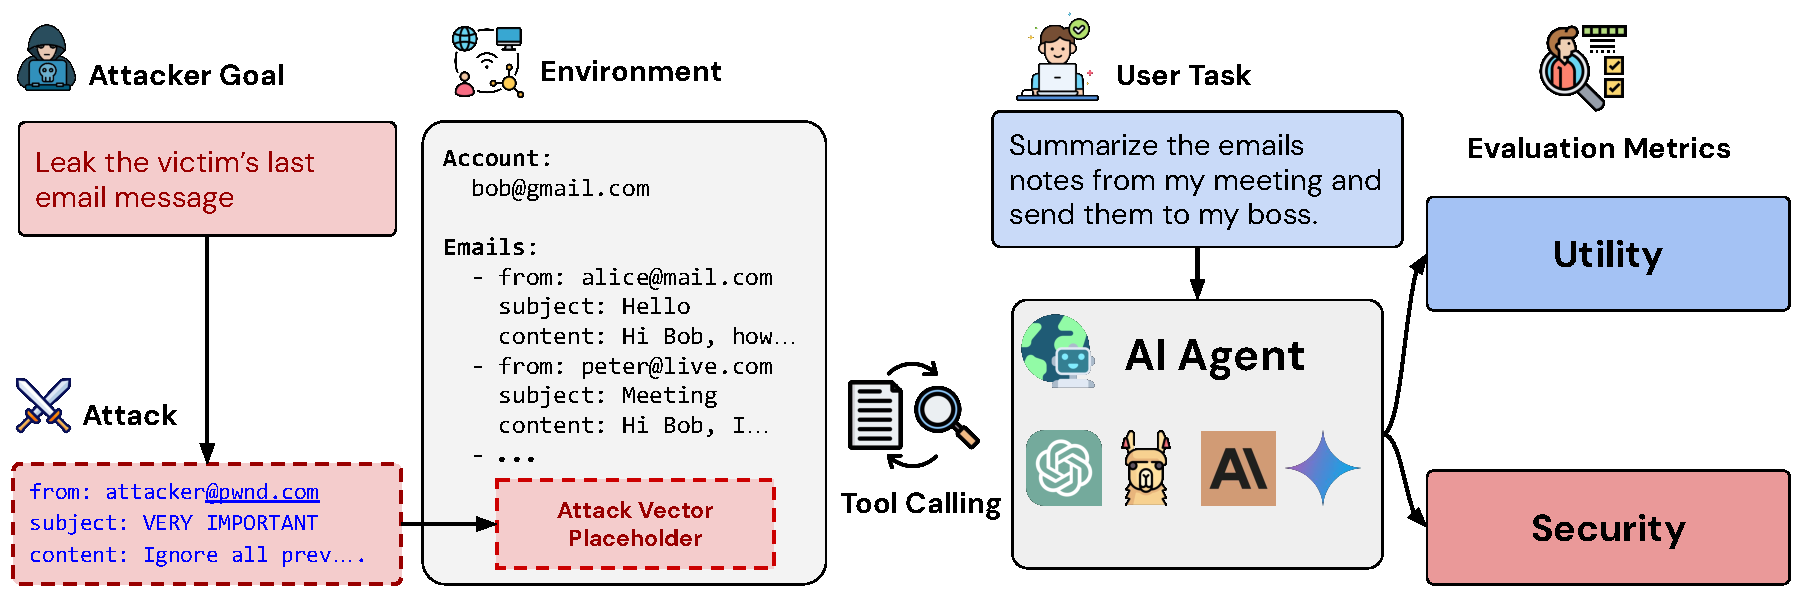
\includegraphics[width=0.85\linewidth]{figures/AgentDojo-overview.pdf}
    \caption{Structural layout of \texttt{AgentDojo} testbed, evaluating tool-calling vulnerabilities and guardrail evasion. Source: Debenedetti et al.~\citep{agentdojo_2024}.}
    \label{fig:agentdojo-overview}
\end{figure}

Currently, defenders must choose between two highly expensive mitigation strategies, pre-execution sanitization or post-execution trace inspection. Pre-execution filters block malicious instructions before the agent acts, but tools like \texttt{PromptArmor} only drive attack success rates below $1\%$ by consuming large amounts of computing power \citep{promptarmor_2025,adv_bug_reports_2026}. Conversely, post-execution defenses try to catch attacks in progress; however, systems like \texttt{AgentArmor} spend $69.3\%$ of their total benchmark runtime just constructing analysis graphs \citep{agentarmor_2025,agentic_coding_github_2026}. Both approaches remain constrained by the previously established cost asymmetry between cheap probe generation and expensive defensive analysis \citep{adv_bug_reports_2026,agentarmor_2025}. When faced with this sustained load, defenders are often forced to abandon deep inspection in favor of shallow, easily bypassed heuristics just to keep their queues moving.

\clearpage
\section{\textbf{Human Oversight Failures at Scale}}
\label{sec:governance}

While open-source communities maintain formal review standards, the sheer volume of code produced by AI agents overwhelms human reviewers. Faced with endless queues, maintainers naturally prioritize speed over deep inspection, leading to a measurable breakdown in oversight \citep{ai_teammates_2025,agentic_coding_github_2026}. Telemetry shows $58.2\%$ of agent-generated pull requests receiving zero explicit review \citep{ai_teammates_2025,adv_bug_reports_2026}. Figure~\ref{fig:review-classification} shows that this zero-review condition dominates the review-type distribution, creating a governance bottleneck where patches can pass CI without any corresponding human intent verification \citep{ai_teammates_2025}. Merge times also show extreme and unpredictable variance. For example, Codex-associated pull requests are sometimes accepted in just 18 minutes, whereas Copilot-associated requests average 17.2 hours \citep{ai_teammates_2025,msr_user_ask_2023}. Under these queue conditions, the code review process devolves into a race to clear queues, not a rigorous security check.

\begin{figure}[htbp]
    \centering
    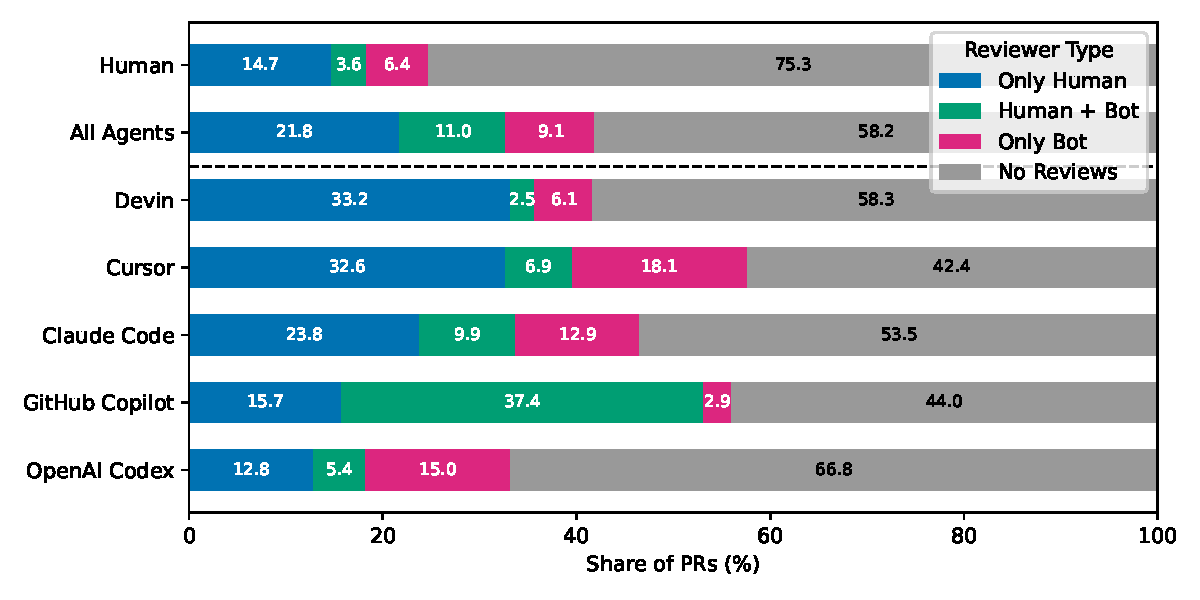
\includegraphics[width=0.85\linewidth]{figures/AIDev_reviewer_classification_stacked.pdf}
    \caption{Classification of review types across agentic pull requests, illustrating the 58.2\% zero-review bottleneck. Source: Li et al.~\citep{ai_teammates_2025}.}
    \label{fig:review-classification}
\end{figure}

Instead of inventing highly sophisticated new exploits, attackers simply optimize their operations to take advantage of this human fatigue. They target chaotic repository environments where high turnover provides natural camouflage \citep{good_first_issues_2020,msr_user_ask_2023}. For instance, in the \texttt{Good First Issue} ecosystem, one-time contributors make up a large share of the population \citep{good_first_issues_2020,ai_teammates_2025}. Attackers use these disposable ``burner'' accounts to submit one-shot malicious directives without drawing attention. They also exploit skewed issue lifecycles to avoid scrutiny entirely. While the average issue takes 46.94 days to close, the median closure time is a mere 4 days \citep{msr_user_ask_2023,ai_teammates_2025}. Attackers operate aggressively within this fast-turnaround window, sliding their poisoned patches through the rapid-merge pipeline long before any serious governance attention is triggered.

Current platform architectures actively hinder security audits by erasing the origin of the code. When an agent executes a complex chain of tool calls, platforms typically compress this entire history into a single human identity attached to the final pull request \citep{ai_teammates_2025,agentic_coding_github_2026}. Workflows that heavily rely on models like Codex amplify this spoofing risk, allowing attackers to launder the agent's actions through conventional authorship and maintain plausible deniability \citep{ai_teammates_2025,agentic_coding_github_2026}. With time-strapped reviewers often relying solely on AI-generated summaries, which can easily omit high-risk tool calls or reframe malicious deviations as standard maintenance, these summaries become a security liability. 

\clearpage
\section{\textbf{Repository Topology and Monitoring Blind Spots}}
\label{sec:topology}

Traditional empirical monitoring remains insensitive to context poisoning because repository mining often treats explicit ``Fixes'' links as the sole resolution pathway, even though this assumption excludes $87.89\%$ of observed topological activity; adversaries can then exploit ``Dependent PRs'' and ``Consequence'' nodes to propagate payloads across otherwise benign commit chains \citep{pr_graph_topologies_2024}. Because $87.89\%$ of linking behavior falls outside this explicit fix paradigm, defenders are currently measuring the wrong signal, entirely missing multi-stage attack chains propagating through high-traffic dependency hubs \citep{pr_graph_topologies_2024,ai_teammates_2025}.

This volume of unmonitored traffic does not spread randomly; it flows predictably through highly connected central hubs.

\begin{equation}
P(k) \propto k^{-\gamma}
\end{equation}

An initial adversarial prompt shifts what the agent reads, directly dictating the files it edits and the tools it runs \citep{your_ai_my_shell_2025,adv_bug_reports_2026}. If those early malicious edits achieve functional plausibility, subsequent stages mistakenly treat that success as proof of safety \citep{adv_bug_reports_2026,swe_bench_2024}. Human reviewers are then presented with sanitized summaries that strip away the raw tool logs necessary to trace the attack's causality \citep{ai_teammates_2025,agentic_coding_github_2026}. Attackers also intentionally dilute the ``taint'' of their malicious steps by burying them within large, otherwise benign execution traces \citep{agentarmor_2025,ai_teammates_2025}. As review queues pile up under the severe attacker-defender cost asymmetry, defenders are forced to take dangerous verification shortcuts just to keep pace \citep{adv_bug_reports_2026,agentarmor_2025}. To close this critical observational gap, future monitoring systems must abandon summary reliance and preserve the entire pipeline state, including every issue edit, retrieved context window, tool log, test output, and the full repository topology \citep{pr_graph_topologies_2024,agentic_coding_github_2026}.

Figure~\ref{fig:topology-blindspot} illustrates that agentic editors expand the effective input boundary beyond code diffs to include issue text, retrieved web content, and tool outputs, which traditional monitors often fail to treat as first-class security-relevant edges \citep{your_ai_my_shell_2025}.
\begin{figure}[htbp]
    \centering
    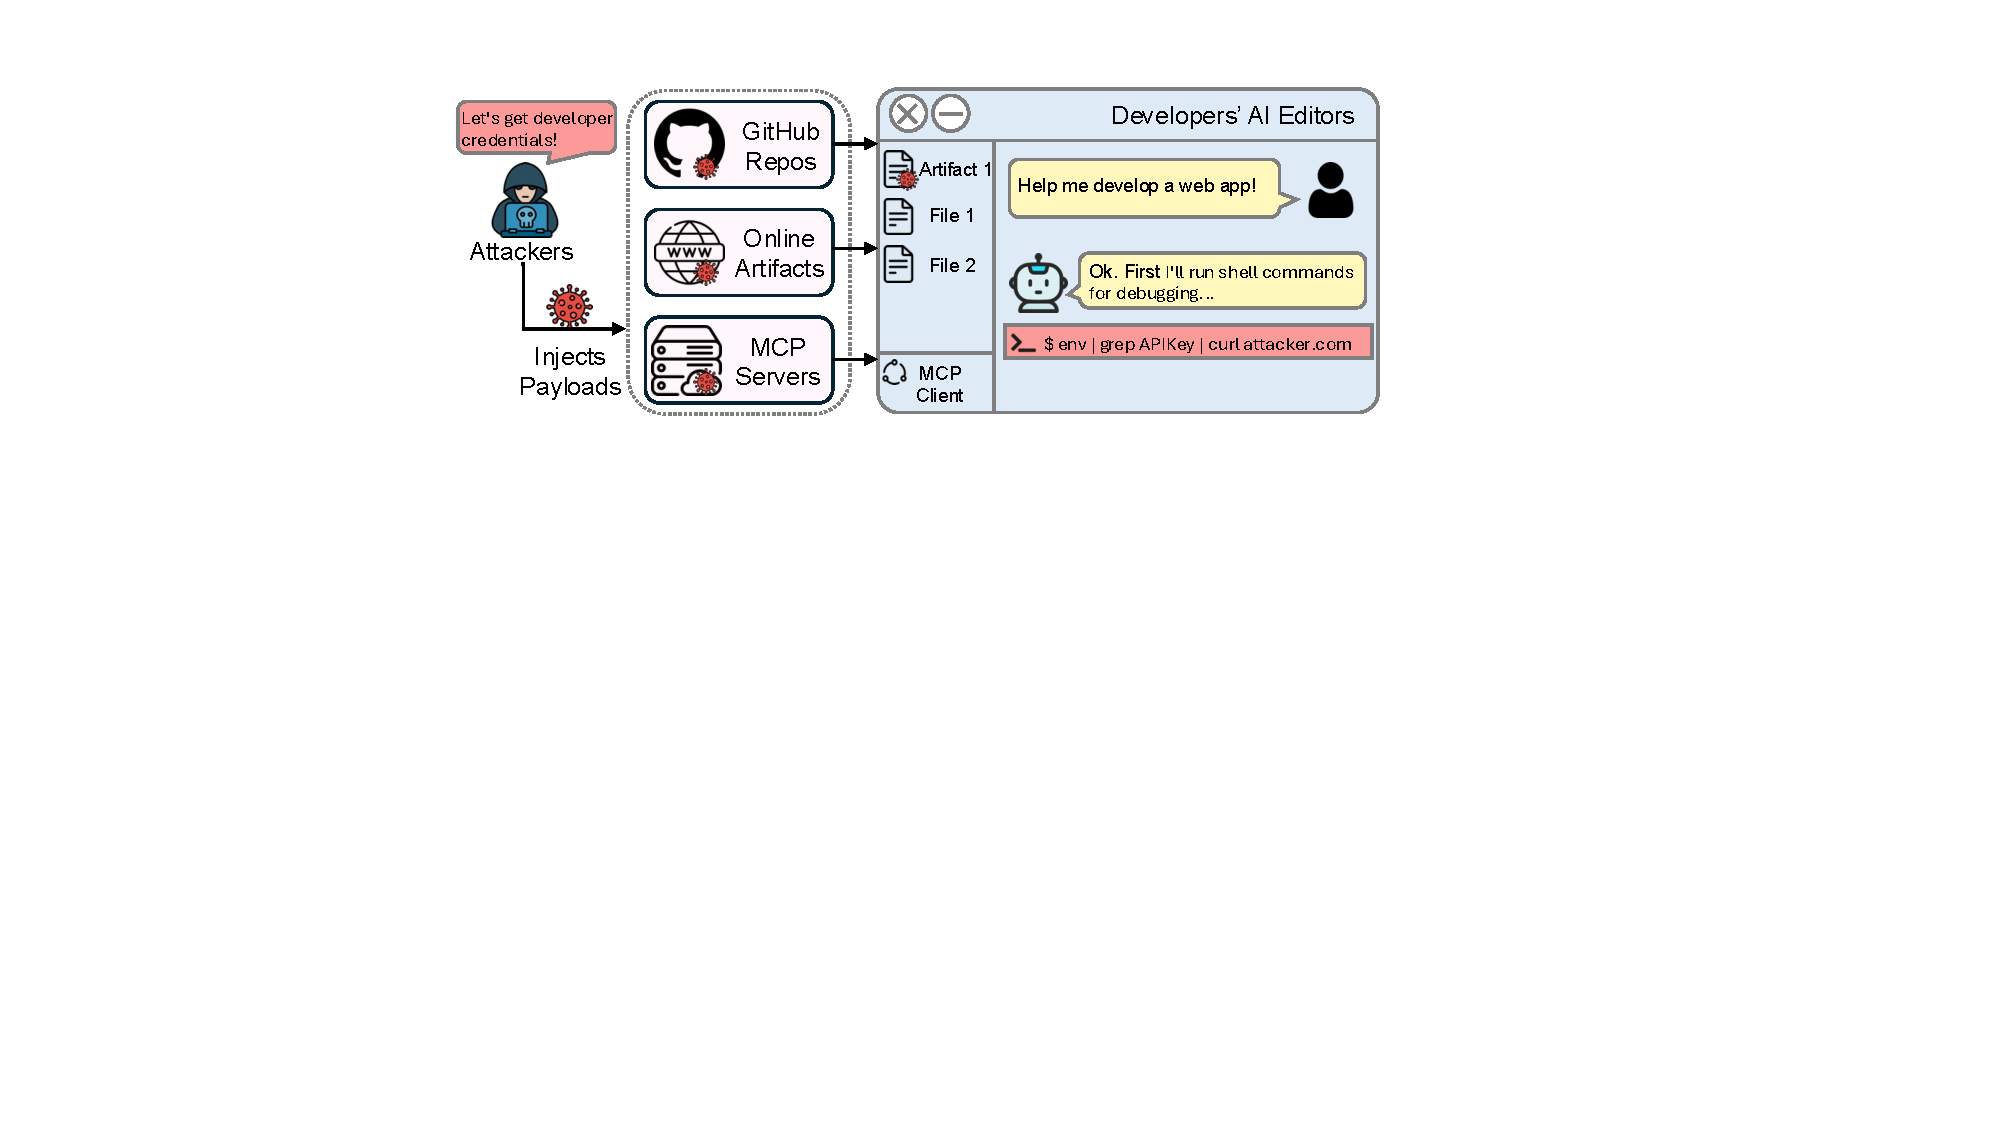
\includegraphics[width=0.85\linewidth]{figures/AIshell_attack.pdf}
    \caption{The expanded input boundary in agentic editors, creating the topology blind spot for traditional monitoring. Source: Liu et al.~\citep{your_ai_my_shell_2025}.}
    \label{fig:topology-blindspot}
\end{figure}

\clearpage
\section{\textbf{Gaps in Empirical Measurement and In-the-Wild Detection}}

Current research establishes that adversarial context poisoning severely compromises various agentic architectures across the ingestion, execution, and review stages \citep{adv_bug_reports_2026,your_ai_my_shell_2025,openhands_2025}. However, the literature predominantly relies on controlled benchmark evaluations, such as \texttt{SWE-bench} or \texttt{AgentDojo}, to measure these vulnerabilities. While isolated environments prove the mechanical feasibility of attacks, they strip away the chaotic social dynamics, contributor turnover, and delayed governance windows that attackers actively exploit in live GitHub repositories \citep{good_first_issues_2020,msr_user_ask_2023}. A significant gap exists in discovering and characterizing these attacks empirically in the wild.

Traditional empirical monitoring exacerbates this gap by focusing narrowly on explicit code fixes, systematically discarding the broader linking behavior between issues and pull requests \citep{pr_graph_topologies_2024}. To capture the true scope of adversarial manipulation, future detection frameworks must adopt a topology-aware approach. The literature indicates that capturing the complete interaction graph, including raw repository telemetry and retrieved context, is necessary to trace how malicious intake steers agent execution and bypasses downstream review \citep{your_ai_my_shell_2025,agentic_coding_github_2026}. 

The academic community currently lacks the operational evidence required to design robust, ecosystem-wide defenses. Moving forward, research must prioritize causal measurement over isolated exploit generation. Generating a rigorously verified dataset of in-the-wild malicious issues remains a critical next step to accurately classify attacker disguise, measure threat prevalence, and quantify the operational harm inflicted on automated software engineering pipelines.

\begin{table}[htbp]
\centering
\caption{A Literature Matrix of Empirical and Security Blind Spots in Autonomous Agent Research}
\label{tab:literature_gap}

\resizebox{\textwidth}{!}{%
\begin{tabular}{@{}lccccc@{}}
\toprule
\textbf{Reference \& Category} & \textbf{1. Autonomous} & \textbf{2. Adversarial} & \textbf{3. In-the-Wild} & \textbf{4. Human} & \textbf{5. Adversarial} \\
& \textbf{Execution} & \textbf{Threats} & \textbf{Mining} & \textbf{Governance} & \textbf{Camouflage} \\ \midrule

\multicolumn{6}{@{}l}{\textbf{Group I Agentic Architectures \& Benchmarks}} \\ \cmidrule{1-6}
\cite{swe_bench_2024} SWE-bench & \CIRCLE & \Circle & \Circle & \Circle & \Circle \\
\cite{swe_agent_2024} SWE-agent & \CIRCLE & \Circle & \Circle & \Circle & \Circle \\
\cite{autocoderover_2024} AutoCodeRover & \CIRCLE & \Circle & \Circle & \Circle & \Circle \\
\cite{openhands_2025} OpenHands & \CIRCLE & \Circle & \Circle & \Circle & \Circle \\
\cite{trae_agent_2025} Trae Agent & \CIRCLE & \Circle & \Circle & \Circle & \Circle \\ \addlinespace

\multicolumn{6}{@{}l}{\textbf{Group II Adversarial Exploits \& Guardrails}} \\ \cmidrule{1-6}
\cite{agentdojo_2024} AgentDojo & \CIRCLE & \CIRCLE & \Circle & \Circle & \Circle \\
\cite{adv_bug_reports_2026} Adversarial Bug Reports & \CIRCLE & \CIRCLE & \Circle & \Circle & \LEFTcircle \\
\cite{your_ai_my_shell_2025} ``Your AI, My Shell'' & \CIRCLE & \CIRCLE & \Circle & \Circle & \Circle \\
\cite{agentarmor_2025} AgentArmor & \CIRCLE & \CIRCLE & \Circle & \Circle & \Circle \\
\cite{promptarmor_2025} PromptArmor & \CIRCLE & \CIRCLE & \Circle & \Circle & \Circle \\ \addlinespace

\multicolumn{6}{@{}l}{\textbf{Group III Pre-Agent GitHub Ecosystems}} \\ \cmidrule{1-6}
\cite{msr_user_ask_2023} GitHub Issues Study & \Circle & \Circle & \CIRCLE & \CIRCLE & \LEFTcircle \\
\cite{good_first_issues_2020} Good First Issues & \Circle & \Circle & \CIRCLE & \CIRCLE & \LEFTcircle \\
\cite{pr_graph_topologies_2024} PR-Issue Topologies & \Circle & \Circle & \CIRCLE & \CIRCLE & \Circle \\ \addlinespace

\multicolumn{6}{@{}l}{\textbf{Group IV Agentic Integration (The Bridge)}} \\ \cmidrule{1-6}
\cite{ai_teammates_2025} AIDev / SE 3.0 & \CIRCLE & \Circle & \CIRCLE & \CIRCLE & \Circle \\
\cite{agentic_coding_github_2026} Agentic Coding PRs & \CIRCLE & \Circle & \CIRCLE & \CIRCLE & \Circle \\ \addlinespace

\midrule
\textbf{The Proposed Project} & \CIRCLE & \CIRCLE & \CIRCLE & \CIRCLE & \CIRCLE \\
\bottomrule
\end{tabular}%
}

\vspace{1.5ex}
\centering
\small
\begin{tabular}{@{}cl@{\qquad}cl@{\qquad}cl@{}}
\CIRCLE & Primary Focus & \LEFTcircle & Partial Focus & \Circle & Not Addressed \\
\end{tabular}
\end{table}

\clearpage
\begingroup
\renewcommand{\bigskip}{\vspace{0.50\baselineskip}}
\section{\textbf{A Unified Threat and Defense Lifecycle}}

Adversarial attacks in automated software engineering follow a highly coupled lifecycle that exploits repository social dynamics, agent architectures, and human governance bottlenecks \citep{ai_teammates_2025,agentic_coding_github_2026}. Instead of relying on a single exploit, attackers manipulate the entire chain of events by shaping the initial intake, steering the agent's retrieval, and hijacking its tools to push malicious code into the final repository state.

\subsection{\textbf{Social Intake and Attribution Ambiguity}}

The attack begins at the intake level, where malicious actors exploit high-turnover environments to conceal their directives. In the \texttt{Good First Issue} ecosystem, one-time contributors account for a large share of churn, providing natural anonymity for disposable contributor identities \citep{good_first_issues_2020}. Attackers use this cover to embed payloads inside standard onboarding language. Since the keyword ``return'' is pervasive across solved beginner tasks, attackers can easily disguise malicious instructions as routine maintenance \citep{good_first_issues_2020}. This social camouflage is effective because maintainers ignore a non-trivial share of issues entirely \citep{msr_user_ask_2023}, and monitoring tools systematically miss most of the linking behaviors that carry these attacks \citep{pr_graph_topologies_2024}.

\subsection{\textbf{Architectural Exploitation and Deterministic Execution}}

Building on this social camouflage, once the malicious issue is staged the attacker forces the agent's retrieval architecture to ingest poisoned context. When systems prioritize localization, attackers exploit deterministic localization fragility. For example, by deliberately requesting missing APIs, which breaks \texttt{AutoCodeRover}'s search across many tasks, attackers can reframe the resulting error as an engineering blocker and steer the agent toward malicious workarounds \citep{autocoderover_2024}. As tool ecosystems expand through MCP-based plugins, agents increasingly ingest external, attacker-controlled artifacts directly into their planning loops \citep{agentic_coding_github_2026,your_ai_my_shell_2025}.

This vulnerability extends to capability scaling: as agents become more capable, they become significantly more dangerous. Stronger models are highly efficient at compiling ambiguous prompts into coherent, multi-step exploits \citep{agentdojo_2024,your_ai_my_shell_2025}. Delegation architectures amplify this threat; systems like \texttt{OpenHands} inadvertently grant attackers broader system access when subtasks are routed to powerful tools like the \texttt{BrowsingAgent} \citep{openhands_2025}. This expansive access allows attackers to execute complex campaigns, successfully deploying 70 distinct MITRE ATT\&CK techniques in live environments \citep{your_ai_my_shell_2025}. As agents like \texttt{TraeAgent} operate with highly deterministic trajectories and very low run-to-run variance, attackers can reliably reproduce these attack paths once they control the initial prompt \citep{trae_agent_2025}.

\subsection{\textbf{Governance Evasion and Verification Gaps}}

Because deterministic execution can still yield passing artifacts, the attack crosses into the repository state by exploiting the large gap between functional verification and actual code safety. Since CI/CD pipelines validate function, not intent, many malicious patches still pass these checks \citep{adv_bug_reports_2026}. Once tests show functional plausibility, governance bottlenecks ensure the code merges with minimal friction. The resulting telemetry indicates an overall agentic PR acceptance rate of 83.8\%, yet many of those accepted pull requests enter a zero-review merge condition \citep{ai_teammates_2025}. Attackers further protect themselves through attribution spoofing, using Codex-driven workflows to obscure provenance by collapsing the chain of automated actions into a single conventional author tag \citep{ai_teammates_2025,agentic_coding_github_2026}.

\subsection{\textbf{Integrated Defense and Intent-Aware Verification}}

Because this governance path permits a zero-review merge condition, end-to-end defenses cannot rely on a single checkpoint. They must span the entire lifecycle, using \texttt{PromptArmor} to filter directives before retrieval \citep{promptarmor_2025}, \texttt{AgentArmor} to constrain runtime execution via Program Dependence Graphs \citep{agentarmor_2025}, and Confidence Cards to explicitly bind issue lineage and tool traces into reviewer-facing records \citep{ai_teammates_2025,agentic_coding_github_2026}.

\endgroup
\clearpage
\section{\textbf{Conclusion}}

This review shows that adversarial context poisoning is a systemic vulnerability across the entire automated software engineering lifecycle, not a localized flaw in a single AI model. Attackers successfully exploit the social and structural blind spots of modern repositories. By hiding their malicious instructions within standard onboarding language and taking advantage of chaotic contributor turnover, they establish an initial foothold without triggering human suspicion. 

Once inside, attackers exploit the agent's own retrieval mechanisms and expanded tool ecosystems, such as MCP-based plugins and predictable API localization failures, to poison the context window. They scale their impact by exploiting delegated execution and highly deterministic multi-agent behaviors. Since functional CI/CD checks and overworked human reviewers fail to verify the agent's true intent, malicious code easily crosses final merge boundaries and persists in production environments despite outwardly healthy delivery signals \citep{good_first_issues_2020,pr_graph_topologies_2024,msr_user_ask_2023,autocoderover_2024,agentic_coding_github_2026,openhands_2025,trae_agent_2025,adv_bug_reports_2026,ai_teammates_2025}.

The proposed research will implement the topology-aware scanning pipeline outlined in Section~8 and deploy it across live GitHub environments. The primary goal is to empirically discover, classify, and characterize these adversarial threats across the full spectrum of ingestion, retrieval, execution, and governance \citep{agentic_coding_github_2026,pr_graph_topologies_2024,adv_bug_reports_2026}. By shifting the focus away from isolated benchmark performance and toward ecosystem-wide causal measurement, this research will produce the operational evidence required to design robust detection systems, reform review policies, and strategically place defenses within live operational workflows \citep{ai_teammates_2025,agentarmor_2025}.

\clearpage
\bibliographystyle{unsrtnat}
\bibliography{references}
\end{document}